\RequirePackage[]{silence}
\WarningFilter{latex}{Marginpar on page}
\WarningFilter{lcg}{Using an already existing counter rand}
\documentclass[article, oneside]{aaltoseries}
\usepackage[utf8]{inputenc}
\usepackage[english]{babel}
\usepackage{IEEEtrantools}
\usepackage[hyphens]{url} % allow hyphens to break urls
\Urlmuskip=0mu  plus 1mu % allow for some spacing inside urls
\usepackage[hidelinks]{hyperref}
\usepackage[acronym]{glossaries}
\usepackage{amsfonts}
\usepackage{todonotes}
\usepackage[normalem]{ulem}
\usepackage{xcolor}
\usepackage{xspace}
\usepackage{textcomp}
\usepackage{etoolbox}
\usepackage[numbers]{natbib}
\newcommand{\TODO}[1]{\todo[inline]{#1}}
\newcommand{\jwnote}[1]{\todo[size=\small,color=blue!40]{#1}}
\newcommand{\JWNOTE}[1]{\todo[size=\small,inline,color=blue!40]{#1}}
\newcommand{\modif}[1]{\textcolor{blue}{#1}}
\newcommand\remove{\bgroup\markoverwith
{\textcolor{red}{\rule[0.5ex]{2pt}{0.8pt}}}\ULon}
\newcommand{\discuss}[1]{\todo[size=\small,color=green!40]{#1}}

\geometry{left=4cm,right=4cm,marginparwidth=3.5cm,marginparsep=5mm} % TODO: remove
% \geometry{left=1cm,right=7cm,marginparwidth=6.5cm,marginparsep=5mm} % TODO: remove
% \reversemarginpar % for todo notes on the wider side

% Use “\tocite{}” to get “citation needed” in document
\newcommand\tocite[1]{
	\todo{\ifstrempty{#1}{Citation needed}{#1}}
	[\,\textbf{\color{red}!}\,]
}


% ************************ Custom Referencing **********************************
\newcommand{\Fref}[1]{Figure~\ref{#1}}
\newcommand{\fref}[1]{figure~\ref{#1}}
\newcommand{\Tref}[1]{Table~\ref{#1}}
\newcommand{\tref}[1]{table~\ref{#1}}
\newcommand{\Eref}[1]{Equation~\ref{#1}}
\newcommand{\eref}[1]{equation~\ref{#1}}
\newcommand{\Sref}[1]{Section~\ref{#1}}
\newcommand{\sref}[1]{section~\ref{#1}}
\newcommand{\Lref}[1]{Listing~\ref{#1}}
\newcommand{\lref}[1]{listing~\ref{#1}}


\newcommand{\app}[1]{A\textsc{pp}$_{#1}$\xspace}

\newacronym{os}{OS}{operating system}
\newacronym{aosp}{AOSP}{Android Open Source Project}

\title{Android App Collusion}


\author{Ervin Oro% Your first and last name: do _not_ add your student number
\\\textnormal{\texttt{ervin.oro@aalto.fi}}} % Your Aalto e-mail address
\affiliation{\textbf{Tutor}: Jorden Whitefield} % First and last name of your tutor

%==========================================================

\begin{document}
\bstctlcite{BSTcontrol}

\maketitle
\todo{set proper margins and document format}
%==========================================================

\begin{abstract}
\TODO{abstract}

\vspace{3mm}
\noindent KEYWORDS: \todo[inline, inlinewidth=5cm, noinlinepar]{list, of, key, words}

\end{abstract}

%============================================================

\section{Introduction}
\label{sec:intro}

Android is an \gls{os} that is primarily designed for mobile devices, e.g., smartphones and tablets. With more than two billion active devices~\cite{AOSP2018}, it is estimated to be the most widely used \gls{os}, surpassing Microsoft Windows~\cite{AWSLLC2018, StatCounter2018}. Android is designed to be an open platform: developed and maintained by Google LLC, but largely released as the \gls{aosp} for everyone to study and evaluate \cite{AOSP2019c}. Android \gls{os} includes support for apps, which are easily installable application packages that can extend the functionality of devices. Apps can be developed and distributed by anyone with very low barrier of entry.

While this popularity of Android is not reflected by the proportion of malware attacks, most of which still target Windows, both the number and complexity of attacks against Android are increasing~\cite{AVTESTGH2018}. This is especially troublesome as many people increasingly rely on their smartphones -- often to store their personal data, online account credentials, money, and more. \citeauthor{McAfee2018} estimates that revenues for mobile malware authors could be in the billion-dollar range by 2020 \cite{McAfee2018}.

Given the increasing potential damage from Android malware, defending against it is an active area of research. Android uses a multi-layer security approach, combining machine learning, platform security and secure hardware~\cite{AOSP2018}. Machine learning methods are utilised by Google Play Store to prevent uploading potentially harmful applications, and by Google Play Protect\footnote{\url{https://www.android.com/play-protect/}}\discuss{citation vs footnote} to scan apps locally on users' devices. Android's platform security has been enhanced over the years with the addition of multiple security features, for example, SELinux protections\footnote{\url{https://source.android.com/security/selinux/}}, exploit mitigations\footnote{\url{https://lwn.net/Articles/695991/}}, privilege reductions\footnote{\url{https://android-developers.googleblog.com/2017/07/seccomp-filter-in-android-o.html}}, and encryption. Recent versions of Android leverage hardware security features, including keystore and remote key attestation\footnote{\url{https://android-developers.googleblog.com/2017/09/keystore-key-attestation.html}}, and receive regular software updates. These security mechanisms have been partially successful, as exploit pricing and difficulty are growing by some estimates~\cite{AOSP2018}.

However, malicious actors are continuously developing exploits to bypass existing protections, and a number of threats, e.g., app collusion, cannot yet be reliably detected nor defended against. App collusion is a secret collaboration between apps with malicious intent  (\Sref{sec:def}). This can be facilitated by any of the numerous ways for apps to communicate with each other that the Android system provides (\Sref{sec:methods}). Methods for apps to collude also exist on the iOS platform \cite{Deshotels2016}. Given a malicious app that would be detected and blocked with state of the art security systems, its functionality can be split into several apps, so that each of them would be categorised as benign when analysed separately~\cite{Chen2018}.

Android app collusion is not a new concept~\cite{Schlegel2011}, and multiple attempts have been made to develop a suitable detection system. \TODO{brief overview of existing approaches based on \Sref{sec:approaches}}
% Filtering
% 	rule-based
% 	machine learning
% model based
% runtime

Despite this, there are currently no robust and usable ways to detect app collusions. Most proposed solutions have a large number of false positives due to their inability to differentiate collusion from legitimate collaboration. Furthermore, since the number of possible combinations is exponential in the number of apps, that is, $N^N$\todo{explain why $N^N$}, most proposed solutions apply very aggressive filtering, causing only some malicious combinations to be included into analysis, and others to be reported as false negatives. \remove{Finally, }approaches attempting to overcome both of these issues have been computationally infeasible thus far. Therefore, app collusion remains an open research challenge.

This report aims to provide an overview of app collusion on the Android platform as follows. \Sref{sec:def} discusses the nature of app collusions in general,~\Sref{sec:methods} provides specific overview of methods that can be used for colluding on Android,~\Sref{sec:examples} describes known examples of colluding apps, and~\Sref{sec:approaches} gives a more in-depth systematic overview of approaches that have been taken to collusion detection and their limitations.

\section{Description and definition of app collusion}
\label{sec:def}

The Oxford English Dictionary defines collusion as ``Secret agreement or understanding for purposes of trickery or fraud; underhand scheming or working with another; deceit, fraud, trickery''~\cite{OEDcollusion}. \citeauthor{Asavoae2017}~\cite{Asavoae2017} define collusion for the case of Android apps as the situation where several apps are working together in performing a threat. According to these definitions, app collusion must have the following three properties:

\begin{enumerate}
	
	\item Colluding apps must be working together secretly. Conversely, apps working together in collaboration is common and encouraged practice when such collaboration is well documented \tocite{}.

	\item All colluding apps must be in agreement. A distinctly different but related concept is the ``confused deputy'' attack, where one app mistakenly exposes itself to other installed apps \tocite{Hardy, N.: The confused deputy:(or why capabilities might have been invented. ACMSIGOPS Operating Systems Review 22(4), 36–38 (1988)}.

	\item Colluding apps must have malicious intent. The intent of Android app collusion would then be to violate one of Android's security goals, which are defined in \cite{AOSP2019} as:
	\jwnote{I also wonder if it is worth mentioning OWASP Mobile top 10	security... \url{https://www.owasp.org/index.php/Mobile\_Top\_10\_2016-Top\_10}}

	\begin{singleenums}
		\item to protect app data, user data, and system resources (including the network),
		\item to provide app isolation from the system, other apps, and the user.
	\end{singleenums}
\end{enumerate}
	
It is important to note that the goal 3(b) is not to enforce isolation, but \remove{merely }to provide isolation for those who require it. As such, apps working together do not automatically violate goal 3(b), but it would be collusion if apps worked together to break isolation with some other non-content app, the system, or the user.

\TODO{many things affect, including non technical}

\TODO{difficult to distinguish}

\TODO{alternative definition \cite{Xu2017}}

\section{Methods for colluding}
\label{sec:methods}

By default, all Android apps run in separate sandboxes~\cite{AOSP2019b}, which are based on user separation by the Linux kernel, and enhanced by SELinux and \texttt{seccomp}~\cite{AOSP2019e}. By default, all communication between sandboxes is blocked~\cite{AOSP2019b}, but apps can open certain communication channels or prevent being separated into different sandboxes altogether. Some channels, so-called overt channels, are designed to be used by apps to communicate, while others, so-called covert channels, utilise functionalities intended for other purposes. All channels discussed below require the participation of both parties, but some researchers have looked into ways to cross sandbox borders unilaterally, therefore breaking the goal 3(b) in \sref{sec:def}~\tocite{}.

\subsection{Overt channels}
\label{sec:overt}

\citeauthor{AOSP2019b} describes channels designed for inter-app communication, such as sandbox sharing and binder, in \cite{AOSP2019b} and \cite{AOSP2019e}.

Apps published by the same entity may share a sandbox. In this case, there are no restrictions for their communication. These apps can use any of the traditional UNIX-type mechanisms, including filesystem, local sockets, or signals.

When apps are running in different sandboxes, the Linux kernel prevents these sandboxed apps from accessing each other's processes or files. In older Android versions, only Linux discretionary access control was used, allowing apps to make their files world-accessible, but newer versions of Android forbid this using SELinux mandatory access control rules. Apps can still use any file-based communication methods when they have permission to access the external storage, but this way users would have some visibility into the fact that such communication channels may be used by the app.

However, Android also provides a method for apps to communicate without any user-granted permission or visibility. This is enabled by a remote procedure call mechanism called binder\todo{revisit after \sref{sec:approaches}: if it discusses more about binder; it needs to be introduces more - a short introduction to Android platform architecture with figure. See \url{https://developer.android.com/guide/platform}}. Any app can send messages to the binder arbitrarily, but other apps must explicitly start listening and accept incoming communications. The Android platform provides three main ways to do this:
\begin{enumerate}
	\item Services\tocite{read more}. Apps may start services, which can provide interfaces that are directly accessible using binder.
	\item Intent filters\tocite{read more}. Intents are simple message objects that represents an "intention" to do something. Apps may ask some part of them to be executed when an intent with certain properties matching their filter is initiated.\jwnote{See \url{https://developer.android.com/guide/components/intents-filters}. Include Figure 1. Explicit/implicit intents. Look at warning boxes, some interesting advice.}
	\item ContentProviders\tocite{read more}. Apps can define ContentProviders to expose some of their data.
	\TODO{maybe add something about android platform architecture}
\end{enumerate}

The binder provides an easy way for apps to communicate with each other, promoting openness and allowing separation of concerns. Examples include apps using an intent to ask the camera app to take a photo instead of asking camera control permission, and communication apps allowing other apps to share data through itself. Binder has a well-defined interface that could be monitored.

\subsection{Covert channels}
\label{sec:covert}

In addition to the overt channels, a large amount of covert channels have been discovered. \citeauthor{Marforio2012}~\cite{Marforio2012} propose a classification of communication channels based on whether Application level APIs, \Gls{os} native calls, or Hardware functionalities are utilised. \citeauthor{Al-Haiqi2014}~\cite{Al-Haiqi2014} describe categorising covert channels as either timing or storage channels. However, neither of these approaches provides clear boundaries in all cases nor covers all possible covert channels, which by their nature form an unbounded set. This section provides some examples of covert channels in Android.

\citeauthor{Schlegel2011}~\cite{Schlegel2011} show that any application can change the vibrate setting and use intent filters to be notified every time the setting is changed without requiring specific permissions, therefore demonstrating that apps can create an information channel using the vibrate setting.  Similarly, the volume setting can be used. While apps cannot subscribe to be notified when volume is changed and have to manually check this setting, it has the benefit of having 8 different states, as opposed to the vibrate setting, which is a boolean value. These channels are invisible to users, as long as data transmission does not coincide with audio playback or receiving notifications.

\citeauthor{Marforio2012}~\cite{Marforio2012} describe how data could be exchanged between colluding apps by modifying and monitoring the number of threads, processor usage, and free space on filesystem. While some of the APIs they used have been deprecated \cite{nn2017}, partially similar approaches are possible on modern Android versions as well. For example, free disk space can be queried through the StatFs\#getAvailableBlocksLong() API on latest Android versions \cite{AOSP2019reference}.\todo{signpost novel idea}

The system load can also be measured indirectly to transmit information \cite{Marforio2012}. In this scenario, the transmitting app modulates data payload by varying the load on the system. The Receiving app then repeatedly runs a CPU-intensive computation and measures the time it takes to complete, in order to infer whether or not the transmitting app is loading the system or not. This approach was shown to work even when receiver is just some JavaScript in the browser and not an installed Android app.

Another approach is presented by \citeauthor{Al-Haiqi2014}~\cite{Al-Haiqi2014}, where one app utilises the vibration motor to transmit data, and another app uses the accelerometer readings to receive that data. This is further developed by \citeauthor{Qi2018}~\cite{Qi2018}, who propose covert channels based on user behaviour. Instead of using the vibration motor, a transmitting app could prompt the user to move their phone in certain ways, for example, posing as a rally game where the user needs to turn their phone at specific times based on a track generated by the malicious app.

\TODO{Add a subsection conclusion paragraph}

\section{Examples of Android app collusion}
\label{sec:examples}

A basic example of app collusion (\Fref{fig:sample}) is as follows:
\begin{singleenums}
	\item \app{A} obtains some private information.
	\item \app{A} transmits the information to \app{B} using some overt or covert channel.
	\item \app{B} exfiltrates the information over the internet.
\end{singleenums}

\begin{figure}[h]
	\centering
	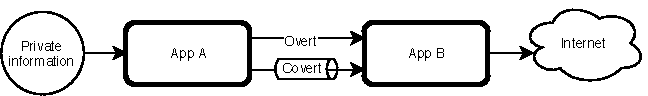
\includegraphics[width=1.0\textwidth]{figures/Collusion1}
	\caption{Structure of a basic app collusion example.}
	\label{fig:sample}
\end{figure}

An early example of this kind of collusion was described by \citeauthor{Schlegel2011}~\cite{Schlegel2011}. In their case, \app{A} was the Soundcomber app that obtained private information using the microphone. To avoid detection, the Soundcomber app did not have permission to access the internet, so they proposed to use a second app to exfiltrate the information. Similar hypothetical example is also described by \citeauthor{Asavoae2017}~\cite{Asavoae2017}, where \app{A} would be a contacts app with READ\_CONTACTS permission, and \app{B} would be a weather app with INTERNET permission.

\TODO{MoPlus SDK}

\section{Existing methods for detecting collusions}
\label{sec:approaches}

%============================================================

\nocite{*}
\bibliographystyle{IEEEtranN}
\bibliography{ieee,oro-cs-seminar}
\TODO{format bibliography}
\TODO{remove nocite}

\listoftodos
\TODO{remove list of todos}

\end{document}
